\documentclass[12pt,letterpaper]{article}
\usepackage{graphicx,textcomp}
\usepackage{natbib}
\usepackage{setspace}
\usepackage{fullpage}
\usepackage{color}
\usepackage[reqno]{amsmath}
\usepackage{amsthm}
\usepackage{fancyvrb}
\usepackage{amssymb,enumerate}
\usepackage[all]{xy}
\usepackage{endnotes}
\usepackage{lscape}
\newtheorem{com}{Comment}
\usepackage{float}
\usepackage{hyperref}
\newtheorem{lem} {Lemma}
\newtheorem{prop}{Proposition}
\newtheorem{thm}{Theorem}
\newtheorem{defn}{Definition}
\newtheorem{cor}{Corollary}
\newtheorem{obs}{Observation}
\usepackage[compact]{titlesec}
\usepackage{dcolumn}
\usepackage{tikz}
\usetikzlibrary{arrows}
\usepackage{multirow}
\usepackage{xcolor}
\newcolumntype{.}{D{.}{.}{-1}}
\newcolumntype{d}[1]{D{.}{.}{#1}}
\definecolor{light-gray}{gray}{0.65}
\usepackage{url}
\usepackage{listings}
\usepackage{color}

\definecolor{codegreen}{rgb}{0,0.6,0}
\definecolor{codegray}{rgb}{0.5,0.5,0.5}
\definecolor{codepurple}{rgb}{0.58,0,0.82}
\definecolor{backcolour}{rgb}{0.95,0.95,0.92}

\lstdefinestyle{mystyle}{
	backgroundcolor=\color{backcolour},   
	commentstyle=\color{codegreen},
	keywordstyle=\color{magenta},
	numberstyle=\tiny\color{codegray},
	stringstyle=\color{codepurple},
	basicstyle=\footnotesize,
	breakatwhitespace=false,         
	breaklines=true,                 
	captionpos=b,                    
	keepspaces=true,                 
	numbers=left,                    
	numbersep=5pt,                  
	showspaces=false,                
	showstringspaces=false,
	showtabs=false,                  
	tabsize=2
}
\lstset{style=mystyle}
\newcommand{\Sref}[1]{Section~\ref{#1}}
\newtheorem{hyp}{Hypothesis}

\title{Problem Set 2}
\date{Due: February 18, 2024}
\author{Applied Stats II}


\begin{document}
	\maketitle
	\section*{Instructions}
	\begin{itemize}
		\item Please show your work! You may lose points by simply writing in the answer. If the problem requires you to execute commands in \texttt{R}, please include the code you used to get your answers. Please also include the \texttt{.R} file that contains your code. If you are not sure if work needs to be shown for a particular problem, please ask.
		\item Your homework should be submitted electronically on GitHub in \texttt{.pdf} form.
		\item This problem set is due before 23:59 on Sunday February 18, 2024. No late assignments will be accepted.
	%	\item Total available points for this homework is 80.
	\end{itemize}

	
	%	\vspace{.25cm}
	
%\noindent In this problem set, you will run several regressions and create an add variable plot (see the lecture slides) in \texttt{R} using the \texttt{incumbents\_subset.csv} dataset. Include all of your code.

	\vspace{.25cm}
%\section*{Question 1} %(20 points)}
%\vspace{.25cm}
\noindent We're interested in what types of international environmental agreements or policies people support (\href{https://www.pnas.org/content/110/34/13763}{Bechtel and Scheve 2013)}. So, we asked 8,500 individuals whether they support a given policy, and for each participant, we vary the (1) number of countries that participate in the international agreement and (2) sanctions for not following the agreement. \\

\noindent Load in the data labeled \texttt{climateSupport.RData} on GitHub, which contains an observational study of 8,500 observations.

\begin{itemize}
	\item
	Response variable: 
	\begin{itemize}
		\item \texttt{choice}: 1 if the individual agreed with the policy; 0 if the individual did not support the policy
	\end{itemize}
	\item
	Explanatory variables: 
	\begin{itemize}
		\item
		\texttt{countries}: Number of participating countries [20 of 192; 80 of 192; 160 of 192]
		\item
		\texttt{sanctions}: Sanctions for missing emission reduction targets [None, 5\%, 15\%, and 20\% of the monthly household costs given 2\% GDP growth]
		
	\end{itemize}
	
\end{itemize}

\newpage
\noindent Please answer the following questions:

\begin{enumerate}
	\item
	Remember, we are interested in predicting the likelihood of an individual supporting a policy based on the number of countries participating and the possible sanctions for non-compliance.
	\begin{enumerate}
		\item [] Fit an additive model. Provide the summary output, the global null hypothesis, and $p$-value. Please describe the results and provide a conclusion.
		%\item
		%How many iterations did it take to find the maximum likelihood estimates?
		\lstinputlisting[language=R, firstline=14, lastline=21]{PS2.Rmd} 

		\includegraphics[width=0.9\linewidth]{pic1}

		 \noindent \textit{The number of fisher scoring iterations is 4}
	\end{enumerate}
	
	\item
	If any of the explanatory variables are significant in this model, then:
	\begin{enumerate}
		\item
		For the policy in which nearly all countries participate [160 of 192], how does increasing sanctions from 5\% to 15\% change the odds that an individual will support the policy? (Interpretation of a coefficient)
%		\item
%		For the policy in which very few countries participate [20 of 192], how does increasing sanctions from 5\% to 15\% change the odds that an individual will support the policy? (Interpretation of a coefficient)
	\lstinputlisting[language=R, firstline=28, lastline=43]{PS2.Rmd}
	 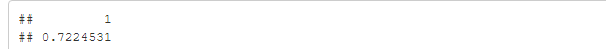
\includegraphics[width=0.9\linewidth]{pic}\\
	\noindent For the policy in which very few countries participate [20 of 192]
	 	\lstinputlisting[language=R, firstline=28, lastline=43]{PS2.Rmd}
		\item
		What is the estimated probability that an individual will support a policy if there are 80 of 192 countries participating with no sanctions? 
			\lstinputlisting[language=R, firstline=68, lastline=71]{PS2.Rmd}
		\noindent The value for the prob is:\\
		 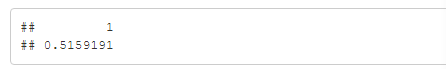
\includegraphics[width=0.9\linewidth]{pic3}\\
		\item
		Would the answers to 2a and 2b potentially change if we included the interaction term in this model? Why? 
		\begin{itemize}
			\item Perform a test to see if including an interaction is appropriate.
			\lstinputlisting[language=R, firstline=77, lastline=81]{PS2.Rmd}
			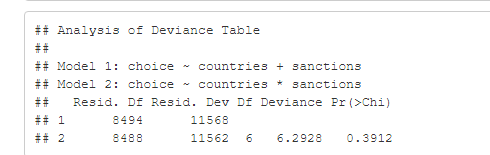
\includegraphics[width=0.9\linewidth]{pic4}\\
			\noindent Including an interaction term in the model could potentially change my answers to questions 2a and 2b because it allows for the effect of one variable (e.g., sanctions) on the response (e.g., support for the policy) to depend on the level of another variable (e.g., number of participating countries). This means that the impact of increasing sanctions could be different depending on how many countries are participating. \\		
			\noindent The code I've written calculates odds ratios for changes in sanctions without considering potential interactions between sanctions and the number of countries. If an interaction term were included in the model, I would need to adjust the `predict` function calls to account for this interaction when estimating probabilities for specific scenarios. This could lead to different probabilities (and therefore different odds and odds ratios) than those calculated without the interaction term, as it would capture more complex relationships between variables.
		\end{itemize}
		
	\end{enumerate}
	\end{enumerate}


\end{document}
